\documentclass[border=2pt,tikz]{standalone}
\usepackage{tikz}
\usepackage{amsmath}
\usepackage{amssymb}

\begin{document}

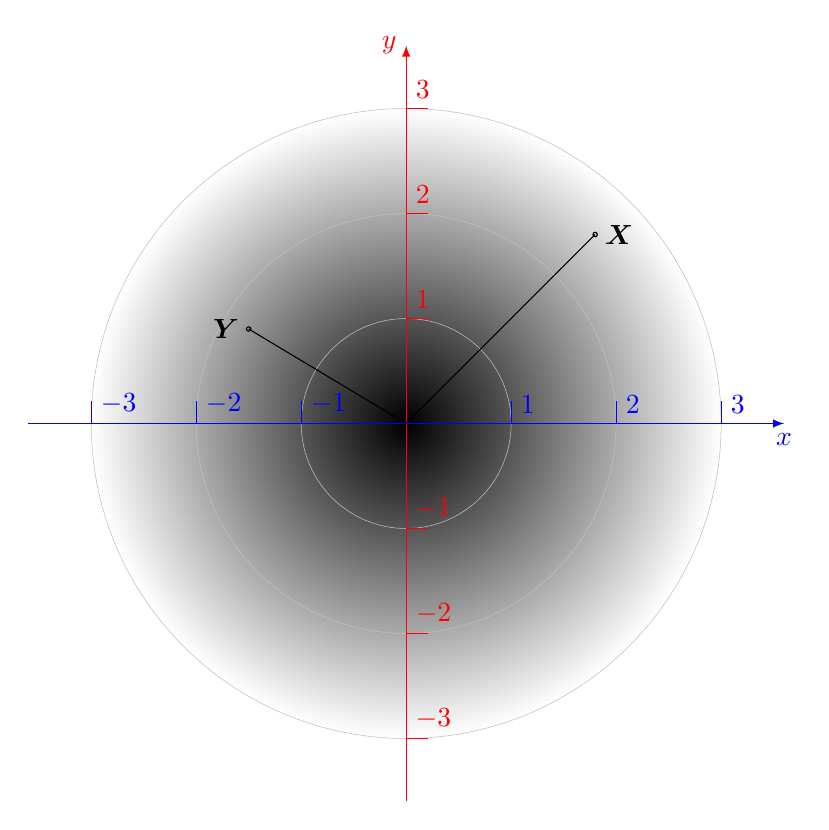
\begin{tikzpicture}[scale=4]

% Draw a circle at the origin of radius 1
\draw [very thin, lightgray, inner color=black!100, outer color=black!0] (0,0) circle (1);
\draw [very thin, lightgray] (0,0) circle (1/3);
\draw [very thin, lightgray] (0,0) circle (1/3*2);

% Draw x and y axis lines
\draw [->,>=latex, color=blue] (-1.2,0) -- (1.2,0) node [below] {$x$};
\draw [->,>=latex, color=red ] (0,-1.2) -- (0,1.2) node [left ] {$y$};

% 画标尺
\foreach \x in {-3, -2, -1, 1, 2, 3}
  \draw [color=blue] (\x/3,2pt) -- (\x/3,0) node [above right] {$\x$};
\foreach \y in {-3, -2, -1, 1, 2, 3}
  \draw [color=red ] (2pt,\y/3) -- (0,\y/3) node [above right] {$\y$};

\draw [->,>=latex] (0,0) -- ( 0.6,0.6) circle (0.2pt) node [right] {$\boldsymbol X$};
\draw [->,>=latex] (0,0) -- (-0.5,0.3) circle (0.2pt) node [left ] {$\boldsymbol Y$};

\end{tikzpicture}

\end{document}

